\documentclass{beamer}

\usepackage{graphicx}
\usepackage{booktabs}
%  \usepackage[T1]{fontenc}
%  \usepackage[latin1]{inputenc}
\usepackage[french]{babel}
\usepackage{algorithm2e}

\mode<presentation> {
	% \usetheme{default}
	% \usetheme{AnnArbor}
	% \usetheme{Antibes}
	% \usetheme{Bergen}
	% \usetheme{Berkeley}
	% \usetheme{Berlin}
	% \usetheme{Boadilla}
	% \usetheme{CambridgeUS}
	% \usetheme{Copenhagen}
	% \usetheme{Darmstadt}
	% \usetheme{Dresden}
	% \usetheme{Frankfurt}
	% \usetheme{Goettingen}
	% \usetheme{Hannover}
	% \usetheme{Ilmenau}
	% \usetheme{JuanLesPins}
	% \usetheme{Luebeck}
	\usetheme{Madrid}
	% \usetheme{Malmoe}
	% \usetheme{Marburg}
	% \usetheme{Montpellier}
	% \usetheme{PaloAlto}
	% \usetheme{Pittsburgh}
	% \usetheme{Rochester}
	% \usetheme{Singapore}
	% \usetheme{Szeged}
	% \usetheme{Warsaw}

	% \usecolortheme{albatross}
	% \usecolortheme{beaver}
	% \usecolortheme{beetle}
	% \usecolortheme{crane}
	% \usecolortheme{dolphin}
	% \usecolortheme{dove}
	% \usecolortheme{fly}
	% \usecolortheme{lily}
	% \usecolortheme{orchid}
	% \usecolortheme{rose}
	% \usecolortheme{seagull}
	% \usecolortheme{seahorse}
	% \usecolortheme{whale}
	% \usecolortheme{wolverine}

	% \setbeamertemplate{footline} % To remove the footer line in all slides uncomment this line
	% \setbeamertemplate{footline}[page number] % To replace the footer line in all slides with a simple slide count uncomment this line
	\setbeamertemplate{navigation symbols}{} % To remove the navigation symbols from the bottom of all slides uncomment this line
}

\AtBeginSection[]{
	\begin{frame}
		\frametitle{Table des matières}
		\tableofcontents[currentsection]
	\end{frame}
}
\AtBeginSubsection[]{
	\begin{frame}
		\frametitle{Table des matières}
		\tableofcontents[currentsubsection]
	\end{frame}
}

\title[État des lieux]{Plate-forme d'entrainement de gestion de crise}
\author{Brandon Alves}
\institute[INSA Lyon]{
	INSA Lyon \\
	\medskip
	INRIA
}
\date{14 Juin 2021}

\begin{document}
	\begin{frame}
		\titlepage
	\end{frame}
	\begin{frame}
		\frametitle{Table des matières}
		\tableofcontents
	\end{frame}
	\section{Architecture du SI existante}
		\begin{frame}
			\frametitle{Architecture du SI existante}
			\begin{block}{Clients}
				\begin{itemize}
					\item client1 (Debian 10)
					\item admin (Debian 10)
				\end{itemize}
			\end{block}
			\begin{block}{Serveurs}
				\begin{itemize}
					\item web (Debian 9)
					\begin{itemize}
						\item dans DMZ
						\item LAMP
					\end{itemize}
					\item mail (Debian 9)
					\begin{itemize}
						\item Poste.io
					\end{itemize}
					\item dns (Debian 9)
					\begin{itemize}
						\item BIND
					\end{itemize}
				\end{itemize}
			\end{block}
		\end{frame}
		\begin{frame}
			\frametitle{Architecture du SI existante}
			\begin{block}{Routeur}
				\begin{itemize}
					\item pfsense (Freebsd)
					\item 5 interfaces (internet, administration, dmz, clients, services)
					\item Firewall pfSense
					\item DHCP
				\end{itemize}
			\end{block}
			\begin{block}{Attaquant}
				\begin{itemize}
					\item attacker (Debian 9)
					\item dans l'internet
					\item dispose de scripts permettant de lancer différentes attaques
				\end{itemize}
			\end{block}
		\end{frame}
		\begin{frame}
			\frametitle{Architecture du SI existante}
			\begin{center}
				\begin{figure}
					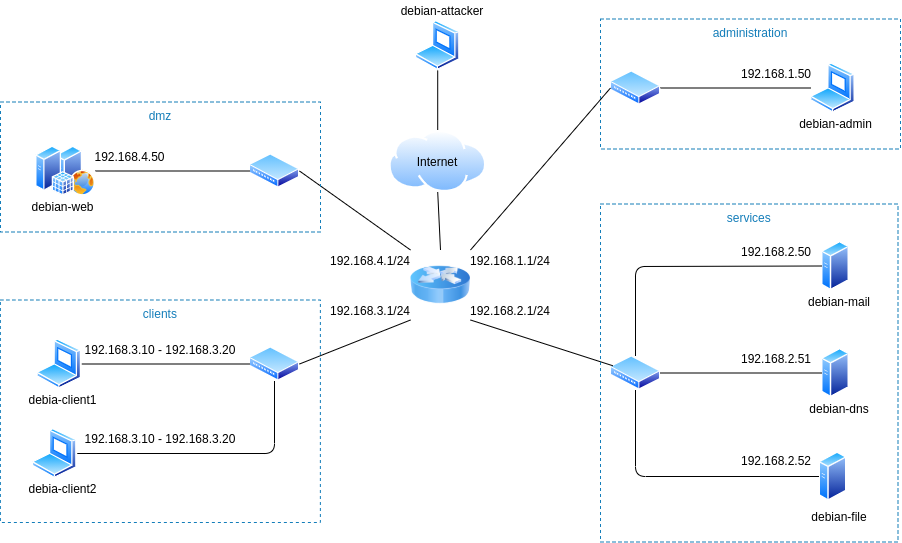
\includegraphics[scale=.3]{si.png}
					\caption{Architecture du SI}
				\end{figure}
			\end{center}
		\end{frame}
		\section{Attaques existantes}
		\begin{frame}
			\frametitle{Attaques existantes}
			\begin{itemize}
				\item Attaque SSH par force brute
				\item Attaque par déni de service (x2 dont \textit{Slowloris})
			\end{itemize}
		\end{frame}
		\section{Informations}
		\begin{frame}
			\frametitle{Comptes utilisateurs}
			\begin{block}{Sur chaque machine : 1 compte}
				\begin{itemize}
					\item login = $<$nom de la machine$>$
					\item password = password
				\end{itemize}
			\end{block}
		\end{frame}
		\begin{frame}
			\frametitle{NAT}
			\begin{center}
				\begin{figure}
					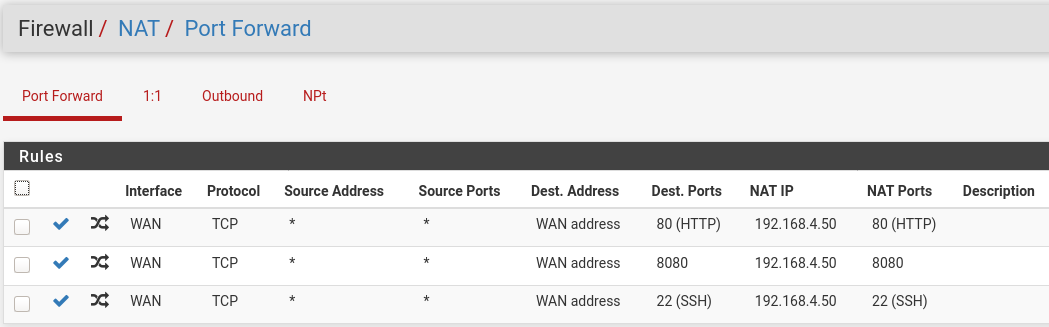
\includegraphics[scale=.3]{portforwading.png}
					\caption{NAT}
				\end{figure}
			\end{center}
		\end{frame}
		\begin{frame}
			\frametitle{Règles}
			\begin{center}
				\begin{figure}
					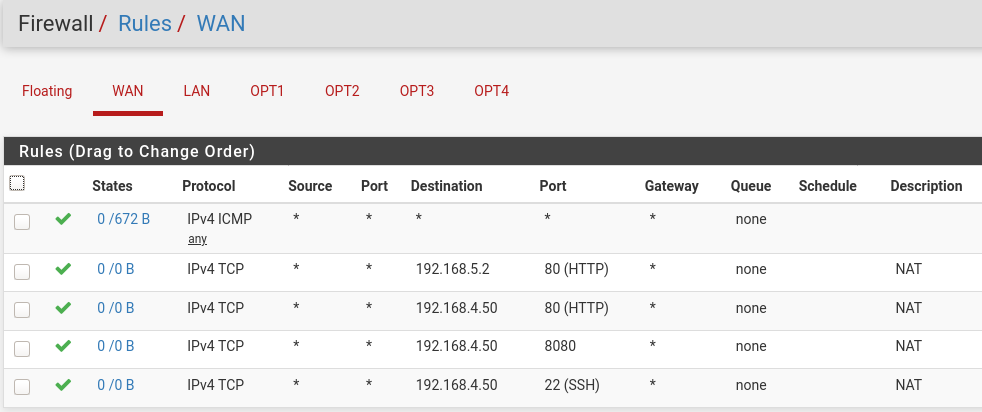
\includegraphics[scale=.3]{rules.png}
					\caption{}
				\end{figure}
			\end{center}
		\end{frame}
		\begin{frame}
			\frametitle{Règles}
			\begin{center}
				\begin{figure}
					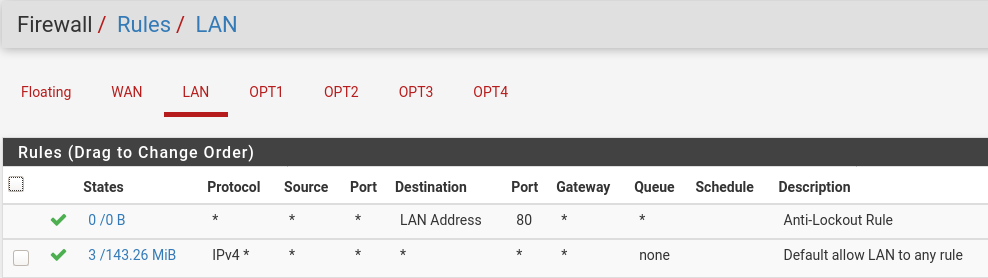
\includegraphics[scale=.3]{rules2.png}
					\caption{}
				\end{figure}
			\end{center}
		\end{frame}
		\begin{frame}
			\frametitle{Règles}
			\begin{center}
				\begin{figure}
					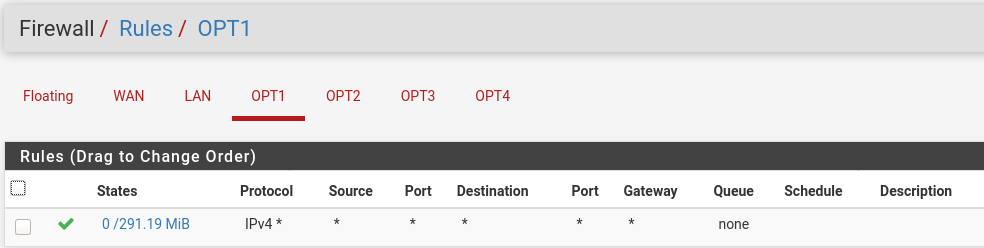
\includegraphics[scale=.3]{rules3.png}
					\caption{}
				\end{figure}
			\end{center}
		\end{frame}
		\section{Sujet summer school}
		\begin{frame}
			\frametitle{Sujet summer school}
			\begin{block}{Description}
				\begin{itemize}
					\item FrenchLeather SA
					\item tannerie
					\item région Lyonnaise
					\item travail comporte des risques pour les employés
					\item conditions de travail difficiles
					\item produits toxiques plus aventageux économiquement que produits bios
				\end{itemize}
			\end{block}
		\end{frame}
		\begin{frame}
			\frametitle{Sujet summer school}
			\begin{block}{On peut imaginer \ldots}
				\begin{itemize}
					\item vente en ligne $\rightarrow$ seveur web $\rightarrow$ DoS
					\item adresses de messagerie professionnel $\rightarrow$ piratage du compte du patron $\rightarrow$ chantage
					\item serveur de fichier ? des photos du patron avec sa maitresse ? $\rightarrow$ l'attaquant arrive à s'y introduire récupère les images et fait chanter
					\item serveur de base de données $\rightarrow$ contient : CA, nb de bléssés, salaire, employés non déclarés, \ldots
				\end{itemize}
			\end{block}
		\end{frame}
		\begin{frame}
			\frametitle{Sujet summer school}
			\begin{block}{Autres attaques}
				\begin{itemize}
					\item injection SQL sur le site web de l'entreprise
					\item phishing par mail
					\item ransomeware sur des données sensibles
					\item spyware
				\end{itemize}
			\end{block}
		\end{frame}
	\begin{frame}
		\begin{itemize}
			\item \url{https://www.oodrive.com/fr/blog/securite/top-10-differents-types-cyberattaques/}
			\item \url{https://zeltser.com/malware-sample-sources/}
		\end{itemize}
	\end{frame}
\end{document}
